\documentclass[letterpaper]{article}

%% Language and font encodings
\usepackage[english]{babel}
\usepackage[utf8x]{inputenc}
\usepackage[T1]{fontenc}

%% Sets page size and margins
\usepackage[letterpaper, margin=0.75in]{geometry}

%% Useful packages
\usepackage{amsmath}
\usepackage{graphicx}
\usepackage[colorinlistoftodos]{todonotes}
\usepackage[colorlinks=true, allcolors=blue]{hyperref}
\usepackage{listings}
\usepackage{xcolor}
\usepackage{fancyvrb, newverbs, color}

\lstnewenvironment{Python}
  {\lstset{language=Python,frame=single}}
  {}
\lstnewenvironment{CPP}
  {\lstset { %
    language=C++,
    frame=single,
    basicstyle=\footnotesize,% basic font setting
    keywordstyle=\color{blue}\ttfamily,
    stringstyle=\color{red}\ttfamily,
    commentstyle=\color{green}\ttfamily,
    morecomment=[l][\color{magenta}]{\#}
  }}
  {}

\title{Udacity Flying Car Nanodegree 4th Project\\ 
       Build an Estimator in C++}
\author{Xinjie Qiu \\
        qiuxinjie@gmail.com}
\date{\today}

\begin{document}
\maketitle

\section{Introduction}

The purpose of this project is to develope and implement Extended Kalman Filter used by a controller to estimate the state of a flight vehicle from realistic sensors in the C++ simulator. 


The math that is useful to implement EKF is provided by Udacity in the \href{https://www.overleaf.com/read/vymfngphcccj}{Estimation for Quadrotors} document.

\section{Project Structure}

\begin{itemize}
  \setlength\itemsep{0em}
  \item The EKF to implement is in \href{https://github.com/tjphoton/FCND/blob/master/FCND-P4-Estimation-CPP/src/QuadEstimatorEKF.cpp}{QuadEstimatorEKF.cpp} in the src directory.
  \item Parameters for tuning the EKF are in the parameter file \href{https://github.com/tjphoton/FCND/blob/master/FCND-P4-Estimation-CPP/config/QuadEstimatorEKF.txt}{QuadEstimatorEKF.txt} in the config directory.
  \item Re-tuned controller \href{https://github.com/tjphoton/FCND/blob/master/FCND-P4-Estimation-CPP/src/QuadControl.cpp}{QuadController.cpp} and \href{https://github.com/tjphoton/FCND/blob/master/FCND-P4-Estimation-CPP/config/QuadControlParams.txt}{QuadControlParams.txt} to work successfully with the implemented estimator.
\end{itemize}

\section{Implement Estimator}

\subsection{Sensor Noise}

In real drone, sensor measurement is never perfect. There must be some noise associated with the sensor readings. In this step, some simulated noisy sensor data were collected from a static quad to estimate the standard deviation of the quad's sensor.

\begin{figure}[ht]
\centering
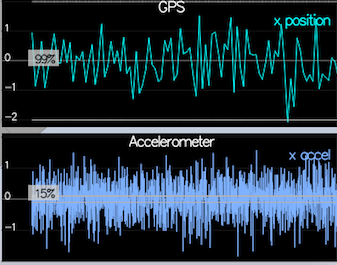
\includegraphics[width=0.5\textwidth]{./images/noise1.png}
\caption{\label{fig:noise1} Noise in the GPS posiiton and IMU Accelerometer position measurement with some arbitrary bound.}
\end{figure}

In scenario 6 NoisySensors simulation, displayed in Figure~\ref{fig:noise1} are two plots, one for GPS X position and one for The accelerometer's x acceleration measurement. 

The dashed lines are a visualization of an arbitrary chosen standard deviation from 0 for each signal. The standard deviation chosen for GPS X position measurement is so large that it encloses 99\% of the measurement. The standard deviation chosen for IMU Accelerometer X acceleration measurement is so small that it only encloses 15\% of the measurement. Our task is to calculate the correct standard deviation for each sensor that should enclose ~68\% of the sensor measurements.

the collected data are recorded to the following csv files with headers: 
\begin{itemize}
  \setlength\itemsep{0em}
  \item config/log/Graph1.txt (GPS X data),
  \item config/log/Graph2.txt (IMU Accelerometer X data).
\end{itemize}

Calculate standard deviation of the the GPS X signal and the IMU Accelerometer X signal from these two logged files with the following Python code:

\begin{Python}
import pandas as pd
import numpy as np

gps_x  = pd.read_csv('./config/log/Graph1.txt')
imu_ax = pd.read_csv('./config/log/Graph2.txt')

gps_x_std  = np.std(gps_x[' Quad.GPS.X'])
imu_ax_std = np.std(imu_ax[' Quad.IMU.AX'])

print('GPS position std is {0:.2f}'.format(gps_x_std))
print('IMU accelerometer position std is {0:.2f}'.format(imu_ax_std))
\end{Python}

\begin{Verbatim}[frame=lines, label=Calculation Result Output, commandchars=\\\{\}]
GPS x position std is \textcolor{red}{0.72}
IMU x accelerometer std is \textcolor{red}{0.51}
\end{Verbatim}

Plug in the result into the top of config/6\_Sensornoise.txt to set MeasuredStdDev\_GPSPosXY and MeasuredStdDev\_AccelXY to be the values just calculated.

\begin{Python}
MeasuredStdDev_GPSPosXY = 0.72
MeasuredStdDev_AccelXY = 0.51
\end{Python}

\begin{figure}[ht]
\centering
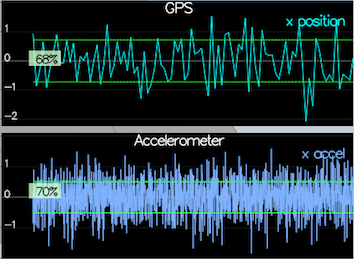
\includegraphics[width=0.5\textwidth]{./images/noise2.png}
\caption{\label{fig:noise2} Noise in the GPS posiiton and IMU Accelerometer position measurement with $\pm 1 \sigma$ bound.}
\end{figure}

Run the simulator again with corrected values, the dashed lines in Fig~\ref{fig:noise2} in the simulation eventually turn green, indicating capturing approx 68\% of the respective measurements, which is what we should expect within $\pm 1 \sigma$ for a Gaussian noise model.

These calculated values also match the settings in SimulatedSensors.txt, where you can also grab the simulated noise parameters for all the other sensors.

\begin{Verbatim}[frame=single, commandchars=\\\{\}]
[SimIMU]
AccelStd = \textcolor{red}{.5, .5}, 1.5
GyroStd = .5, .5, .5
dt = .002

[SimGPS]
PosStd = \textcolor{red}{.7, .7}, 2
#PosRandomWalkStd = .1, .1, .1
VelStd = .1, .1, .3
dt = .1
\end{Verbatim}

\subsection{Attitude Estimation}

In this step, we will include information from IMU and use complementary filters in stead of Kalman filter for our attitude state estimation.

The vehicle's attitude state, $x_t$ consists pitch $\theta$ and roll $\phi$.
\begin{align*}
  x_t = \left[ \begin{array}{c}\theta\\\phi \end{array} \right]
\end{align*}

The observation, $z_t$ consists angles pitch $\theta$ and roll $\phi$ as estimated from the accelerometer in the global frame, and the angular velocity $p$ and $q$ from the gyro in the body frame.
\begin{align*}
  z_t = \left[ \begin{array}{c}\theta\\\phi\\p\\q \end{array} \right]
\end{align*}

Since the pitch and roll angles obtained by an accelerometer have large noises but a small drift, while pitch and roll angles estimated by integrating angular velocity from gyro sensor have a little noise but a large drift, a linear complementary filter expressed below can obtain a more accurate attitude estimation, due to high-frequency noise attenuated after passing the low-pass filter, and the low-frequency signal be eliminated after passing the high-pass filter.

For pitch: 
\begin{align*}
  \hat{\theta}_t = \frac{\tau}{\tau + T_s} \left( \hat{\theta}_{t-1} + T_s z_{t,\dot{\theta}} \right) + \frac{T_s}{\tau + T_s} z_{t,\theta}
\end{align*}

Similarly for roll: 

\begin{align*}
  \hat{\phi}_t = \frac{\tau}{\tau + T_s} \left( \hat{\phi}_{t-1} + T_s z_{t,\dot{\phi}} \right) + \frac{T_s}{\tau + T_s} z_{t,\phi}
\end{align*}

$\tau$ is a time constant and $T_s$ is the filter sampling period:


\subsubsection{Linear Complementary Filter}

Assume that $\theta$ and $\phi$ are small, so that the turn rates measured by the gyro in the body frame approximate the global turn rates,
\begin{align*}
  \left[\begin{array}{c}\dot{\phi}\\\dot{\theta}\\\dot{\psi}\end{array}\right]
  \approx
  \left[\begin{array}{c}p\\q\\r\end{array}\right]  
\end{align*}

This allows us to use a linear complementary filter-type attitude filter, which is already implemented in the function UpdateFromIMU() in QuadEstimatorEKF.cpp, quoted below:

\begin{CPP}
void QuadEstimatorEKF::UpdateFromIMU(V3F accel, V3F gyro)
{
    // SMALL ANGLE GYRO INTEGRATION:

    float predictedPitch = pitchEst + dtIMU * gyro.y;
    float predictedRoll = rollEst + dtIMU * gyro.x;
    ekfState(6) = ekfState(6) + dtIMU * gyro.z;   // yaw

    // normalize yaw to -pi .. pi
    if (ekfState(6) > F_PI) ekfState(6) -= 2.f*F_PI;
    if (ekfState(6) < -F_PI) ekfState(6) += 2.f*F_PI;

    // CALCULATE UPDATE
    accelRoll = atan2f(accel.y, accel.z);
    accelPitch = atan2f(-accel.x, 9.81f);

    // FUSE INTEGRATION AND UPDATE
    rollEst = attitudeTau / (attitudeTau + dtIMU) * predictedRoll +
                  dtIMU / (attitudeTau + dtIMU) * accelRoll;
    pitchEst = attitudeTau / (attitudeTau + dtIMU) * predictedPitch +
                   dtIMU / (attitudeTau + dtIMU) * accelPitch;

    lastGyro = gyro;
}
\end{CPP}

In scenario 7 AttitudeEstimation simulation, IMU is the only sensor used and noise levels are set to 0. There are two plots visible in this simulation in Fig~\ref{fig:linear_comp_filter}. The top graph is showing errors in each of the estimated Euler angles. The bottom shows the true Euler angles and the estimates. There’s quite a bit of error in attitude estimation, ~0.2 rad for yaw, ~0.05 rad for pitch and roll.

\begin{figure}[ht]
\centering
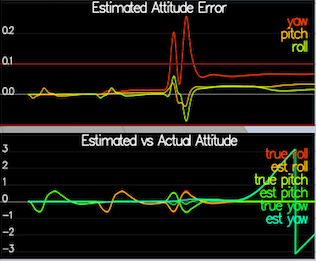
\includegraphics[width=0.5\textwidth]{./images/scenario7_1.png}
\caption{\label{fig:linear_comp_filter} Errors in each of the estimated Euler angles from a linear complementary altitude filter.}
\end{figure}

\subsubsection{Nonlinear Complementary Filter}

We will improve the altitude estimation with implementation of a better non-linear complementary attitude filter using quaternions.

First, we define a quaternion, $q_t$, from the euler angles for $\theta$ , $\phi$ and $\psi$.  The included Quaternion class has a handy Quaternion::FromEuler123\_RPY() function for creating a quaternion from Euler Roll/Pitch/Yaw angles:

\begin{CPP}
// use euler angles to define a quaternion
Quaternion<float> q_t = Quaternion<float>::FromEuler123_RPY(rollEst, pitchEst, ekfState(6));
\end{CPP}

Then the predicted quaternion, $\bar{q}_t$, can be obtained by integrating the measurement of the angular rates from the IMU in the body frame with the included Quaternion class Quaternion::IntegrateBodyRate() function:

\begin{CPP}
// integrate the body rates into a new predicted quaternion
Quaternion<float>  q_t_bar = q_t.IntegrateBodyRate(V3D(gyro.x, gyro.y, gyro.z), dtIMU);
\end{CPP}

Finally we can obtain $\bar{\theta}_t$ and $\bar{\phi}_t$ as follows:

\begin{align*}
  \bar{\theta}_t = Pitch(\bar{q}_t)\\
  \bar{\phi}_t = Roll(\bar{q}_t)
\end{align*}

\begin{CPP}
// extract roll, pitch, yaw from new quaternion
float predictedRoll  = q_t_bar.Roll();
float predictedPitch = q_t_bar.Pitch();
ekfState(6)    = q_t_bar.Yaw();
\end{CPP}

Using these predicated estimates, we can compute the non-linear complementary filter as the same way as above.

For pitch:
\begin{align*}
  \hat{\theta}_t = \frac{\tau}{\tau + T_s} \left( \bar{\theta}_{t-1} + T_s z_{t,\dot{\theta}} \right) + \frac{T_s}{\tau + T_s} z_{t,\theta}
\end{align*}

Similarly for roll: 

\begin{align*}
  \hat{\phi}_t = \frac{\tau}{\tau + T_s} \left( \bar{\phi}_{t-1} + T_s z_{t,\dot{\phi}} \right) + \frac{T_s}{\tau + T_s} z_{t,\phi}
\end{align*}

Put the above pieces together, we have an improved altitude state non-linear complementary filter implementation.
\begin{CPP}
void QuadEstimatorEKF::UpdateFromIMU(V3F accel, V3F gyro)
{
    // Nonlinear Complementary Filter
    // use euler angles to define a quaternion
    Quaternion<float> q_t = Quaternion<float>::FromEuler123_RPY(rollEst, pitchEst, ekfState(6));

    // integrate the body rates into a new predicted quaternion
    Quaternion<float>  q_t_bar = q_t.IntegrateBodyRate(V3D(gyro.x, gyro.y, gyro.z), dtIMU);

    // extract roll, pitch, yaw from new quaternion
    float predictedRoll  = q_t_bar.Roll();
    float predictedPitch = q_t_bar.Pitch();
    ekfState(6)    = q_t_bar.Yaw();

    // CALCULATE UPDATE
    accelRoll = atan2f(accel.y, accel.z);
    accelPitch = atan2f(-accel.x, 9.81f);

    // FUSE INTEGRATION AND UPDATE
    rollEst = attitudeTau / (attitudeTau + dtIMU) * predictedRoll +
                  dtIMU / (attitudeTau + dtIMU) * accelRoll;
    pitchEst = attitudeTau / (attitudeTau + dtIMU) * predictedPitch +
                   dtIMU / (attitudeTau + dtIMU) * accelPitch;

    lastGyro = gyro;
}
\end{CPP}

\begin{figure}[ht]
\centering
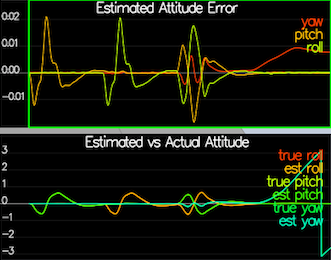
\includegraphics[width=0.5\textwidth]{./images/scenario7_2.png}
\caption{\label{fig:nonlinear_comp_filter} Errors in each of the estimated Euler angles from a non-linear complementary altitude filter.}
\end{figure}

The new non-linear complementary filter reduces the attitude errors from 0.2 rad rad to 0.01 rad for yaw, from 0.05 rad to 0.02 rad for pitch and roll, as shown in the screenshot below in Fig.~\ref{fig:nonlinear_comp_filter}, well within the requirement of 0.1 rad for each of the Euler angles for at least 3 seconds.

\subsection{Implement Filter Prediction}

\subsubsection{Perfect IMU}

Scenario 08 PredictState is configured to use a perfect IMU (only an IMU). 

The state, $x_t$ we are estimating (excluding yaw, which is updated in the IMU update) position and velocity,
\begin{align*}
  x_t = \left[\begin{array}{c} 
      x\\
      y\\
      z\\
      \dot{x}\\
      \dot{y}\\
      \dot{z}\\
      \end{array}\right]
\end{align*}

$u_t$ is the IMU accelerometer measurement in the body frame, indicated by the superscripts $b$. 

\begin{align*}
  u_t &= \left[ \begin{array}{c}
      \ddot{x}^b \\
      \ddot{y}^b \\
      \ddot{z}^b \\
      \end{array} \right]
\end{align*}

To convert acceleration vector from body frame to inertial frame, an attitude Quaternion is created from the current state. 

\begin{CPP}
Quaternion<float> attitude = Quaternion<float>::FromEuler123_RPY(rollEst, pitchEst, curState(6));
\end{CPP}

Then Use Quaternion::Rotate\_BtoI() function to rotate the vector from body frame to inertial frame.
\begin{CPP}
V3F accel_i = attitude.Rotate_BtoI(accel);
\end{CPP}

Finally, in QuadEstimatorEKF.cpp, a simple state prediction is implemented in the PredictState() functon to predict the current state forward by time $dt$ using current velocities and accelerations (already convered in the inertial frame, as indicated by the $i$ superscripts). Since $dt$ will be very short (on the order of 1ms) so simplistic integration methods are fine here.

The prediction function is expressed as,
\begin{align*}
  \left[  \begin{array}{c}
      x_{t+1,x} \\
      x_{t+1,y} \\
      x_{t+1,z} \\
      x_{t+1,\dot{x}} \\
      x_{t+1,\dot{y}} \\
      x_{t+1,\dot{z}} \\
    \end{array}\right] &=
  \left[  \begin{array}{l}
      x_{t,x} + x_{t,\dot{x}} \Delta t \\
      x_{t,y} + x_{t,\dot{y}} \Delta t \\
      x_{t,z} + x_{t,\dot{z}} \Delta t \\
      x_{t,\dot{x}} + \ddot{x}^i  \Delta t \\
      x_{t,\dot{y}} + \ddot{y}^i  \Delta t \\
      x_{t,\dot{z}} + \ddot{z}^i  \Delta t - g \Delta t \\
    \end{array}\right] 
\end{align*}

\newpage

\begin{CPP}
VectorXf QuadEstimatorEKF::PredictState(VectorXf curState, float dt, V3F accel, V3F gyro)
{
    // Predict the current state forward by time dt using current accelerations 
    // and body rates as input
    //
    // INPUTS: 
    //   curState: starting state
    //   dt: time step to predict forward by [s]
    //   accel: acceleration of the vehicle, in body frame, *not including gravity* [m/s2]
    //   gyro: body rates of the vehicle, in body frame [rad/s]
    //   
    // OUTPUT:
    //   return the predicted state as a vector

    assert(curState.size() == QUAD_EKF_NUM_STATES);
    VectorXf predictedState = curState;

    Quaternion<float> attitude = Quaternion<float>::FromEuler123_RPY(rollEst, pitchEst, curState(6));

    // rotates acceleration vector in body coordinate to global coords
    V3F accel_i = attitude.Rotate_BtoI(accel);

    // predict the current state using current accelerations and body rates
    predictedState(0) += curState(3)*dt;
    predictedState(1) += curState(4)*dt;
    predictedState(2) += curState(5)*dt;
    predictedState(3) += accel_i.x*dt;
    predictedState(4) += accel_i.y*dt;
    predictedState(5) += (accel_i.z - CONST_GRAVITY)*dt;

    return predictedState;
}
\end{CPP}

When run scenario 08 PredictState in the simulator, the estimator state track the actual state, with only reasonably slow drift, as shown in the Fig~\ref{fig:perfect_imu} below:

\begin{figure}[ht]
\centering
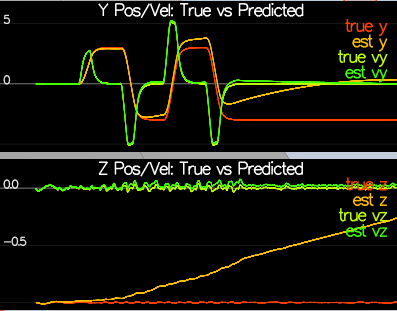
\includegraphics[width=0.5\textwidth]{./images/scenario8_2.png}
\caption{\label{fig:perfect_imu} state prediction with perfect IMU.}
\end{figure}

\subsubsection{Realistic IMU}

Now let's introduce a realistic IMU with noise. In scenario 09 PredictionCov, a small fleet of quadcopter all using your prediction code to integrate forward. There are two plots in Fig~\ref{fig:real_imu}: The top graph shows 10 (prediction-only) position X estimates, the bottom graph shows 10 (prediction-only) velocity estimates. However the estimated covariance (white bounds) currently do not capture the growing errors. This is because the covariance matrix has never been updated. It is always the value set in the QuadEstimatorEKF.txt

\begin{figure}[ht]
\centering
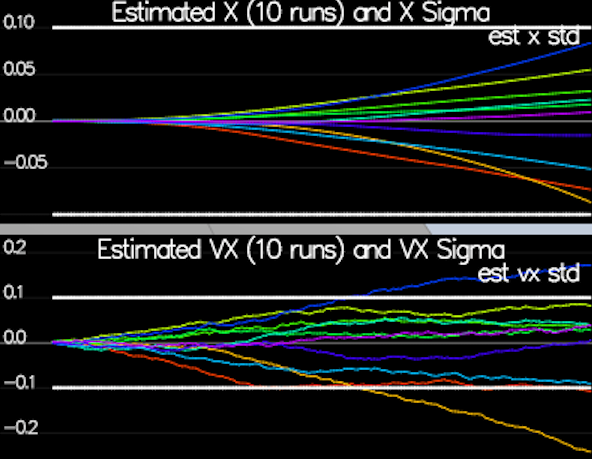
\includegraphics[width=0.5\textwidth]{./images/scenario9_1.png}
\caption{\label{fig:real_imu} State covariance constant prediction for realistic IMU.}
\end{figure}

\begin{Verbatim}[frame=single, commandchars=\\\{\}]
[QuadEstimatorEKF]
InitState = 0, 0, -1, 0, 0, 0, 0
InitStdDevs = \textcolor{red}{.1}, .1, .3, \textcolor{red}{.1}, .1, .3, .05
\end{Verbatim}

To update the covariance matrix to a predicted covariance matrix according to the EKF equation, first a partial derivative of the body-to-global rotation matrix in the function GetRbgPrime() need to be calculated. $R'_{bg}$ is defined as:
\begin{align*}
R'_{bg} = \left[
  \begin{array}{ccc}
    -\cos \theta \sin \psi&
    -\sin\phi \sin \theta \sin \psi - \cos \phi \cos \psi&
    -cos \phi \sin \theta \sin \psi + \sin \phi \cos \psi\\
    \cos \theta \cos \psi&
    \sin \phi \sin \theta \cos \psi - \cos \phi \sin \psi&
    \cos \phi \sin \theta \cos \psi + \sin \phi \sin \psi\\
    0&0&0
  \end{array}
  \right]
\end{align*}

\begin{CPP}
MatrixXf QuadEstimatorEKF::GetRbgPrime(float roll, float pitch, float yaw)
{
    // Return the partial derivative of the Rbg rotation matrix with respect to yaw. 
    // We call this RbgPrime.
    // INPUTS: 
    //   roll, pitch, yaw: Euler angles at which to calculate RbgPrime
    // OUTPUT:
    //   return the 3x3 matrix representing the partial derivative at the given point

    // first, figure out the Rbg_prime
    MatrixXf RbgPrime(3, 3);
    RbgPrime.setZero();

    float cosTheta = cos(pitch);
    float sinTheta = sin(pitch);
    float cosPhi   = cos(roll);
    float sinPhi   = sin(roll);
    float cosPsi   = cos(yaw);
    float sinPsi   = sin(yaw);

    // Fill in matrix elements
    RbgPrime(0,0)  = -cosTheta*sinPsi;
    RbgPrime(0,1)  = -sinPhi*sinTheta*sinPsi - cosTheta*cosPsi;
    RbgPrime(0,2)  = -cosPhi*sinTheta*sinPsi + sinPhi*cosPsi;
    RbgPrime(1,0)  = -cosTheta*cosPsi;
    RbgPrime(1,1)  = sinPhi*sinTheta*cosPsi - cosTheta*sinPsi;
    RbgPrime(1,2)  = cosPhi*sinTheta*cosPsi + sinPhi*sinPsi;
    // the last row of the matrix are all zeros

    return RbgPrime;
}
\end{CPP}

Once $R'_{bg}$ function is implement, the rest of the prediction step to predict the state covariance forward in Predict() is also implemented.

First we take the Jacobian:
\begin{align}
  g'(x_t, u_t, \Delta t) &= 
      \left [ \begin{array}{ccccccc}
      1 & 0 & 0 & \Delta t & 0 & 0 & 0\\
      0 & 1 & 0 & 0 & \Delta t & 0 & 0\\
      0 & 0 & 1 & 0 & 0 & \Delta t & 0\\
      0 & 0 & 0 & 1 & 0 & 0 & R'_{bg}[0:]u_t[0:3] \Delta t\\
      0 & 0 & 0 & 0 & 1 & 0 & R'_{bg}[1:]u_t[0:3] \Delta t\\
      0 & 0 & 0 & 0 & 0 & 1 & R'_{bg}[2:]u_t[0:3] \Delta t\\
      0 & 0 & 0 & 0 & 0 & 0 & 1
    \end{array}
    \right]
\end{align}

Then update covariance according to the classic EKF algorithm update equations to calculate the predictied state covariance in each update step:

$$G_t = g'(x_t, u_t, \Delta t)$$
$$\bar{\Sigma}_t = G_t\Sigma_{t-1}G_t^T + Q_t$$
where $\Sigma_t$ is the state covariance matrix, and $Q_t$ is the transition covariance.

\begin{CPP}
void QuadEstimatorEKF::Predict(float dt, V3F accel, V3F gyro)
{
    // Predict the current covariance forward by dt using the current accelerations 
    // and body rates as input.
    //
    // INPUTS: 
    //   dt: time step to predict forward by [s]
    //   accel: acceleration of the vehicle, in body frame, *not including gravity* [m/s2]
    //   gyro: body rates of the vehicle, in body frame [rad/s]
    //   state (member variable): current state (state at the beginning of this prediction)
    //   
    // OUTPUT:
    //   update the member variable cov to the predicted covariance

    // predict the state forward
    VectorXf newState = PredictState(ekfState, dt, accel, gyro);

    // we'll want the partial derivative of the Rbg matrix
    MatrixXf RbgPrime = GetRbgPrime(rollEst, pitchEst, ekfState(6));

    // an empty Jacobian currently simply set to identity
    MatrixXf gPrime(QUAD_EKF_NUM_STATES, QUAD_EKF_NUM_STATES);
    gPrime.setIdentity();

    gPrime(0,3) = dt;
    gPrime(1,4) = dt;
    gPrime(2,5) = dt;
    gPrime(3,6) = (RbgPrime(0)*accel).sum()*dt;
    gPrime(4,6) = (RbgPrime(1)*accel).sum()*dt;
    gPrime(5,6) = (RbgPrime(2)*accel).sum()*dt;

    ekfCov = gPrime * ekfCov * gPrime.transpose() + Q;

    ekfState = newState;
}
\end{CPP}

Run the implemented EKF covariance prediction and tune the process parameters QPosXYStd to 0.01 and the QVelXYStd to 0.1 in QuadEstimatorEKF.txt to try to capture the magnitude of the error. 

\begin{Verbatim}[frame=single, commandchars=\\\{\}]
# Process noise model
# note that the process covariance matrix is diag(pow(QStd,2))*dtIMU

QPosXYStd = \textcolor{red}{.01}
QVelXYStd = \textcolor{red}{.1}
\end{Verbatim}

In the first part of the plot in Fig~\ref{fig:real_imu_ekf}, our covariance (the white line) grows very much like the data.

\begin{figure}[ht]
\centering
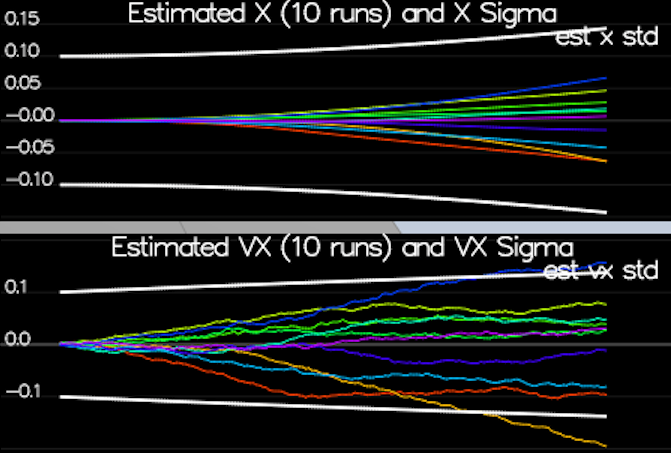
\includegraphics[width=0.5\textwidth]{./images/scenario9_2.png}
\caption{\label{fig:real_imu_ekf} State covariance with EKF prediction for realistic IMU.}
\end{figure}

\subsection{Magnetometer Update}

In the prevous steps, only the accelerometer and gyro sensors were used for the state estimation. In this step, magnetometer sensor measurement is used to estimate the vehicle's heading.

Scenario 10 MagUpdate uses a realistic IMU, but the magnetometer update hasn’t been implemented yet, resulting in the estimate yaw drifting away from the real value. The estimated standard deviation of that state (white boundary) is also increasing. 

Tune the parameter QYawStd to 0.02 in QuadEstimatorEKF.txt for the QuadEstimatorEKF so that it approximately captures the magnitude of the drift, as demonstrated in Fig~\ref{fig:magnetometer}:

\begin{Verbatim}[frame=single, commandchars=\\\{\}]
# Process noise model
# note that the process covariance matrix is diag(pow(QStd,2))*dtIMU

QYawStd = \textcolor{red}{.02}
\end{Verbatim}

\begin{figure}[ht]
\centering
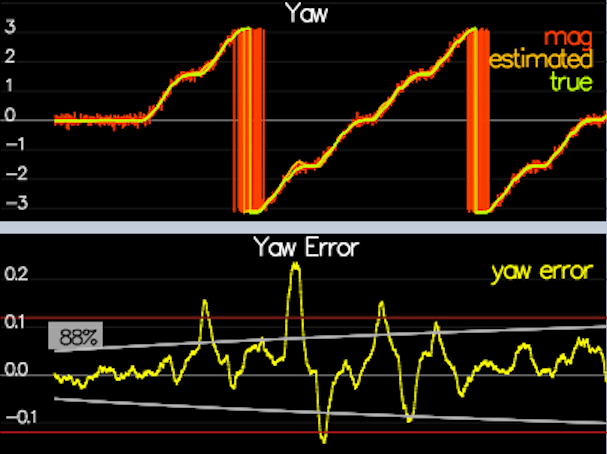
\includegraphics[width=0.5\textwidth]{./images/scenario10_1.png}
\caption{\label{fig:magnetometer} Yaw estimation with no magnetometer update.}
\end{figure}

Now implement magnetometer update in the function UpdateFromMag(). The estimated yaw is the last element in the state vector: ekfState(6).

The reading from the magnetometer $z_t$ reporting yaw in the global frame.
\begin{align*}
  z_t=  \left[\begin{array}{c}
      \psi
      \end{array}\right]
  \end{align*}

a measurement function $h(x_t)$ is defined as,
\begin{align*}
  h(x_t) =  \left[\begin{array}{c}
      x_{t,\psi}
      \end{array}\right]
\end{align*}

$h'(x_t)$ is the Jacobian of $h$ with respect to $x_t$. This Jacobian is a $1 \times 7$ matrix.

\begin{align*}
  h'(x_t) = \left[\begin{array}{ccccccc}
      0&0&0&0&0&0&1
      \end{array}\right]
\end{align*}

The angle error between the current estimated state and the magnetometer measured value is normalized so the update to the yaw would be the short way around the circle, not the long way.

EKF also updates magnetomer measurement covariance R\_Mag, which is a member variable.

The C++ implementation of the magnetometer update:
\begin{CPP}
void QuadEstimatorEKF::UpdateFromMag(float magYaw)
{
    // MAGNETOMETER UPDATE
    VectorXf z(1), zFromX(1);
    z(0) = magYaw;

    MatrixXf hPrime(1, QUAD_EKF_NUM_STATES);
    hPrime.setZero();
     hPrime << 0, 0, 0, 0, 0, 0, 1;

    zFromX(0) = ekfState(6);
    float angle_diff = fmod(zFromX(0) - z(0), (2.0f*(float)M_PI));
    if (angle_diff <= -(float)M_PI)
        zFromX(0) += (2.0f*(float)M_PI);
    else if (angle_diff > (float)M_PI)
        zFromX(0) -= (2.0f*(float)M_PI);

    Update(z, hPrime, R_Mag, zFromX);
}
\end{CPP}

The resulting aaw error plot is in Fig~\ref{fig:magnetometer_update}, with the parameter QYawStd re-tuned to 0.06 to better balance between the long term drift and short-time noise from the magnetometer.


\begin{Verbatim}[frame=single, commandchars=\\\{\}]
# Process noise model
# note that the process covariance matrix is diag(pow(QStd,2))*dtIMU

QYawStd = \textcolor{red}{.06}
\end{Verbatim}

\begin{figure}[ht]
\centering
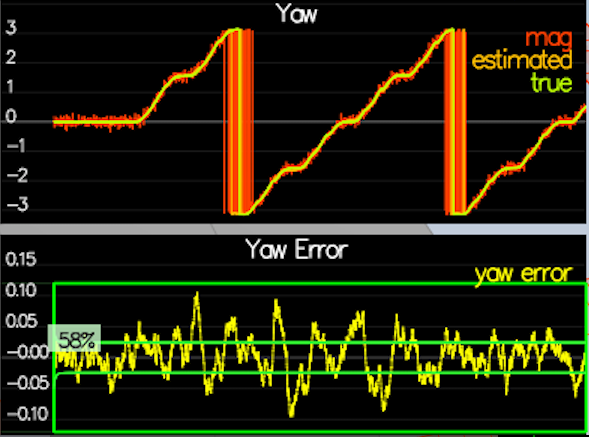
\includegraphics[width=0.5\textwidth]{./images/scenario10_2.png}
\caption{\label{fig:magnetometer_update} Yaw estimation with magnetometer update.}
\end{figure}

\subsection{Closed Loop + GPS Update}

Position and velocity observation are measured from the GPS.

\begin{align*}
  z_t &= \left[ \begin{array}{c}
      x\\
      y\\
      z\\
      \dot{x}\\
      \dot{y}\\
      \dot{z}\\
      \end{array} \right]
\end{align*}

The measurement model is: 
\begin{align*}
  h(x_t) = \left[\begin{array}{c}
      x_{t,x}\\
      x_{t,y}\\
      x_{t,z}\\
      x_{t,\dot{x}}\\
      x_{t,\dot{y}}\\
      x_{t,\dot{z}}\\
    \end{array}\right]
\end{align*}

Jacobian $h'(x_t)$ is the partial derivative of $h(x_t)$, which is a identity matrix, augmented with a vector of zeros for $\frac{\partial}{\partial x_{t,\phi}} h(x_t)$: 
\begin{align*}
  h'(x_t) = \left[\begin{array}{ccccccc}
      1&0&0&0&0&0&0\\
      0&1&0&0&0&0&0\\
      0&0&1&0&0&0&0\\
      0&0&0&1&0&0&0\\
      0&0&0&0&1&0&0\\
      0&0&0&0&0&1&0\\                  
      \end{array}\right]
\end{align*}

Implement the EKF GPS Update in the function UpdateFromGPS():
\begin{CPP}
void QuadEstimatorEKF::UpdateFromGPS(V3F pos, V3F vel)
{
    // GPS UPDATE
    VectorXf z(6), zFromX(6);
    z(0) = pos.x;
    z(1) = pos.y;
    z(2) = pos.z;
    z(3) = vel.x;
    z(4) = vel.y;
    z(5) = vel.z;

    MatrixXf hPrime(6, QUAD_EKF_NUM_STATES);
    hPrime.setZero();
    hPrime.topLeftCorner(6, 6) = MatrixXf::Identity(6, 6);

    zFromX(0) = ekfState(0);
    zFromX(1) = ekfState(1);
    zFromX(2) = ekfState(2);
    zFromX(3) = ekfState(3);
    zFromX(4) = ekfState(4);
    zFromX(5) = ekfState(5);

    Update(z, hPrime, R_GPS, zFromX);
}
\end{CPP}

Tune the process noise model in QuadEstimatorEKF.txt to try to approximately capture the error of the filter. 

Without having to change values of QPosZStd and QVelZStd, the entire simulation cycle can be completed with estimated position error of < 0.4m as shown in Fig~\ref{fig:GPS_update}, less than the < 1m requirement.

Now we have a fulling working estimator!

\newpage

\begin{Verbatim}[frame=single, commandchars=\\\{\}]
# Process noise model
# note that the process covariance matrix is diag(pow(QStd,2))*dtIMU

QPosZStd = \textcolor{red}{.05}
QVelZStd = \textcolor{red}{.1}
\end{Verbatim}

\begin{figure}[ht]
\centering
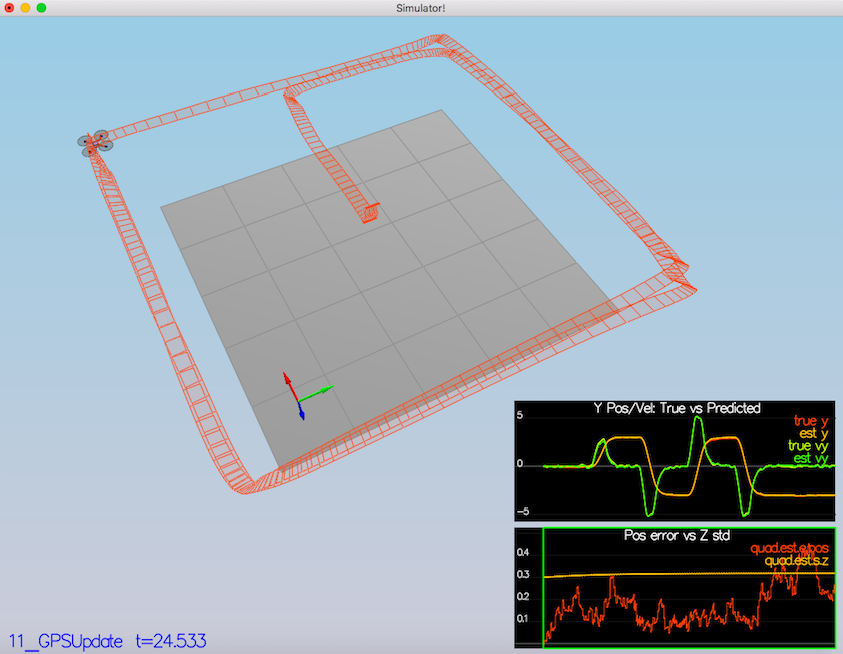
\includegraphics[width=0.8\textwidth]{./images/scenario11.png}
\caption{\label{fig:GPS_update} Position and velocity estimation with GPS update.}
\end{figure}

\section{Adding Previously Implemented Controller}

Replace QuadController.cpp with the controller and uadControlParams.txt with the control parameters from in the last project. Run scenario 11 GPSUpdate, the entire simulation cycle is completed once again with an estimated position error of < 1m, shown in Fig~\ref{fig:GPS_update2}, without de-tuning any control gains.

\begin{figure}[ht]
\centering
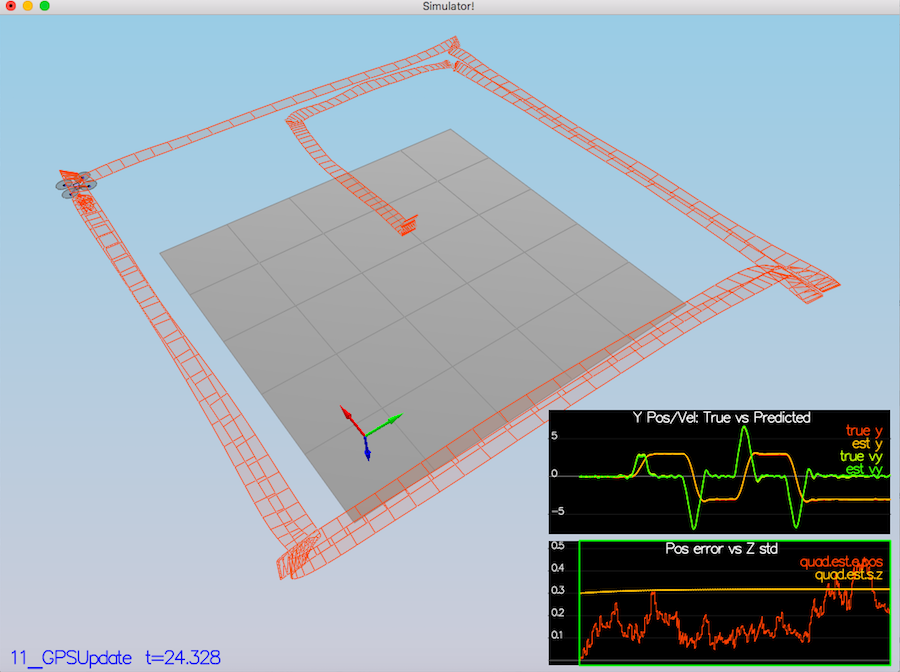
\includegraphics[width=0.8\textwidth]{./images/scenario11_2.png}
\caption{\label{fig:GPS_update2} Position and velocity estimation with GPS update from my previous controller.}
\end{figure}

\clearpage

\section*{Appendix}
This Appendix section is removed, in honor of the appendix being removed from our dear student friend @Luis95014 at 5:30 am on May 27, 2018. Hope he recover well and finish his FCND estimation project soon.

\end{document}